\section{Problem 5}~\label{sec:prob5}

We implement all networks using Parrots.
Codes and training logs can be found at
https://github.com/innerlee/ELEG5491
(Access restricted to campus networks).

\subsection{} % 5.1

The training curve is shown in Figure~\ref{fig:1}.
The learned filters is shown in Figure~\ref{fig:2}.
Comparison between weight decay and no weight decay is shown in Figure~\ref{fig:3}.

\begin{figure}[ht]
\centering
    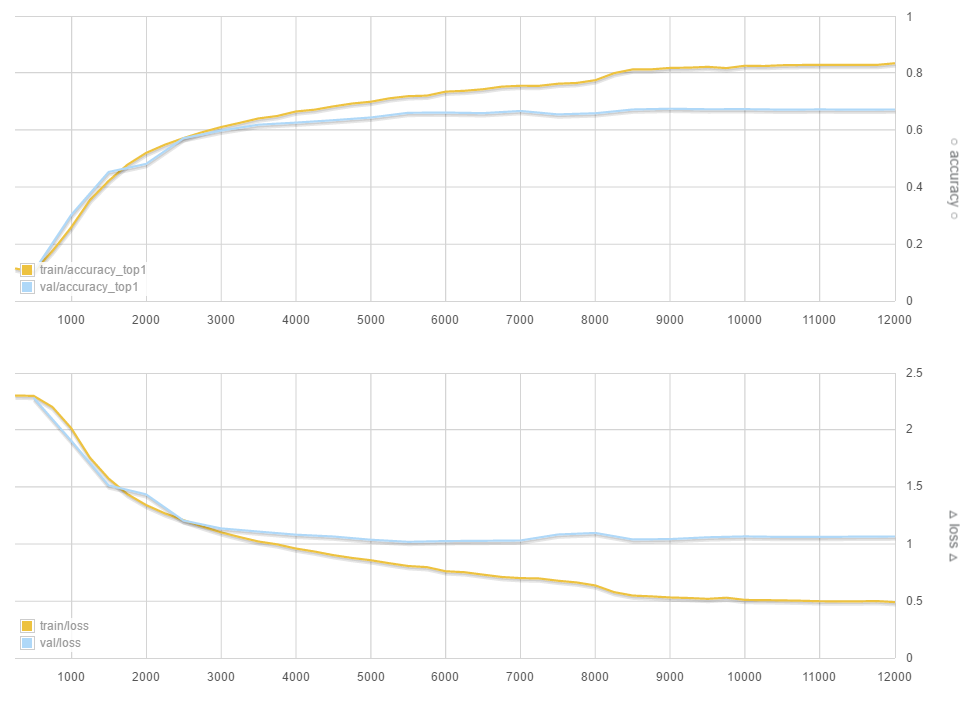
\includegraphics[width=0.99\linewidth]{fig/curve1}
    \caption{\small
    Training curve of the simple network on CIFAR-10.
    initialization is Gaussian.
    The batch size is 256.
    Use SGD as described in the problem.
    The step sizes are 8000, 10000 and 12000.}
    \label{fig:1}
\end{figure}

\begin{figure}[ht]
\centering
    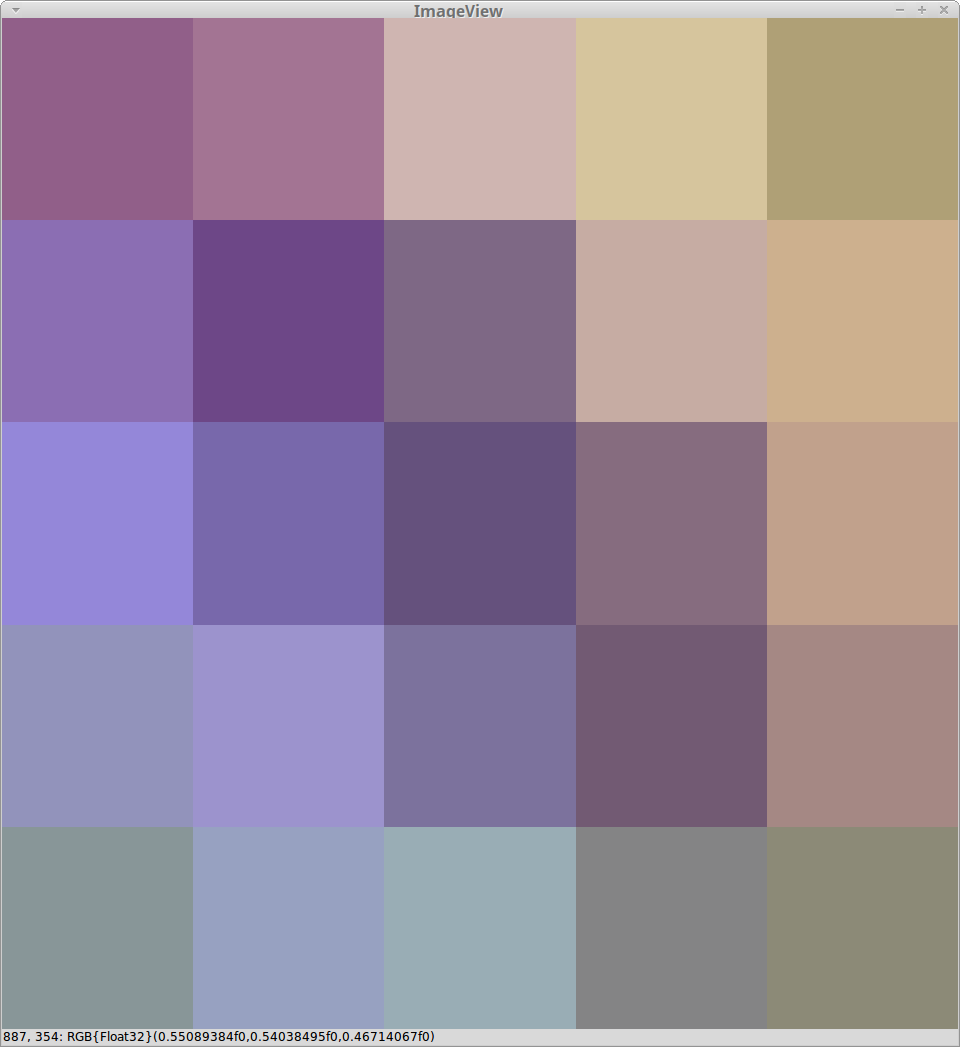
\includegraphics[width=0.3\linewidth]{fig/1}
    
\includegraphics[width=0.3\linewidth]{fig/2}
    
\includegraphics[width=0.3\linewidth]{fig/3}
    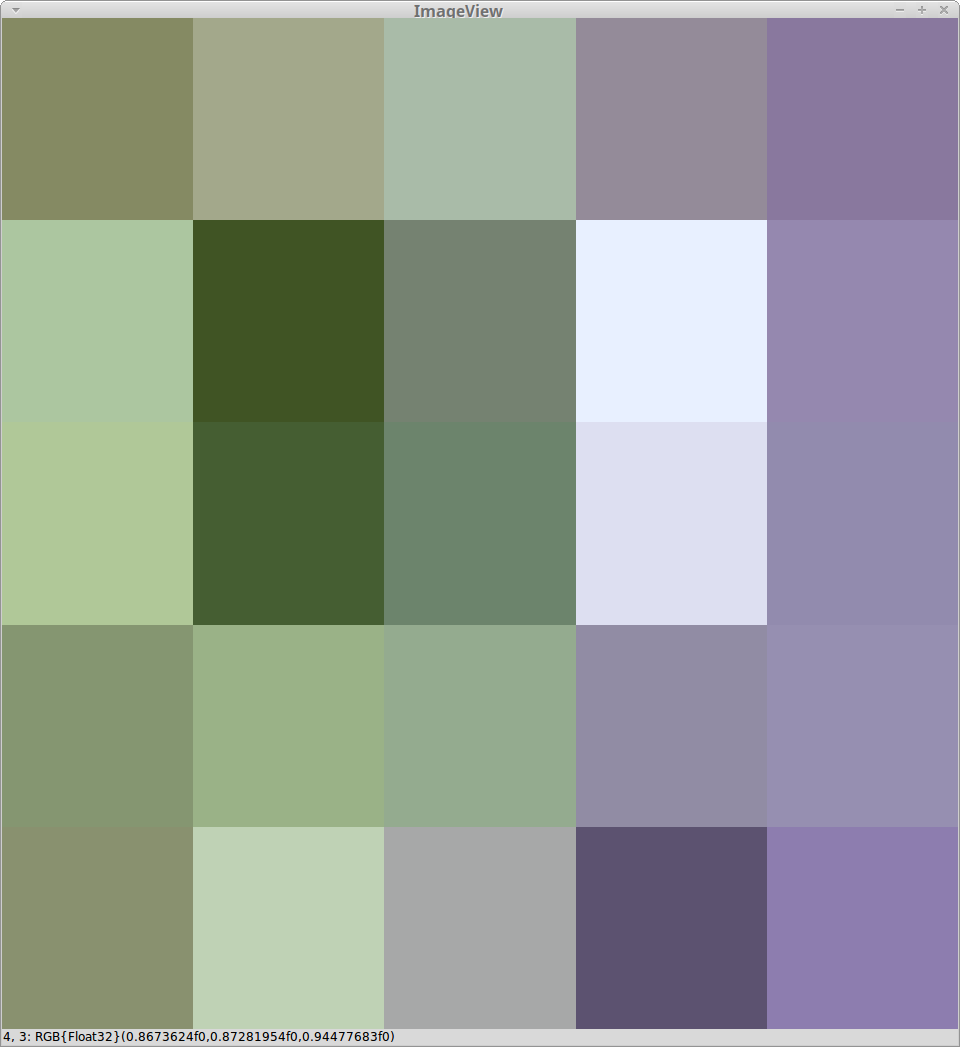
\includegraphics[width=0.3\linewidth]{fig/4}
    
\includegraphics[width=0.3\linewidth]{fig/5}
    
\includegraphics[width=0.3\linewidth]{fig/6}
    \caption{\small
    Visualize the six filters of the first convolutional layer.
    Since the input channel is 3,
    we convert the filters to RGB color images.}
    \label{fig:2}
\end{figure}

\begin{figure}[ht]
\centering
    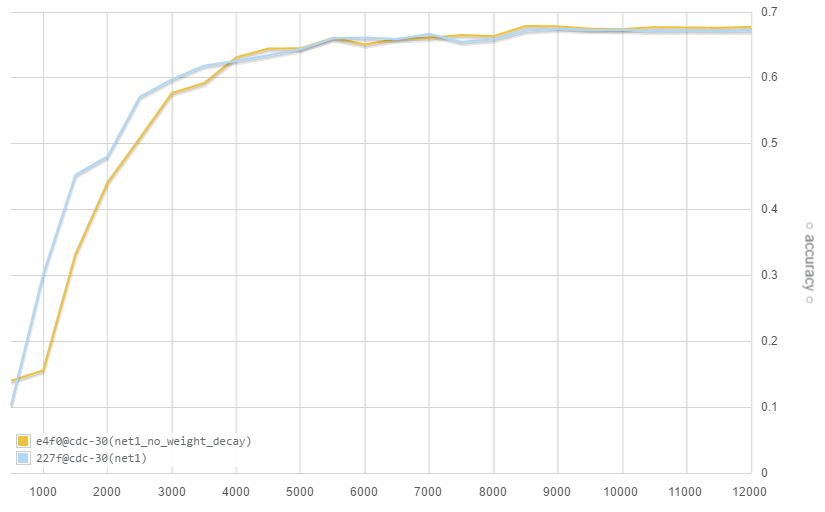
\includegraphics[width=0.9\linewidth]{fig/nodecayacc}
    \caption{\small
    With or without weight decay.
    We can see that they do not have significant difference.
    The one with weight decay has best val accuracy $67.44\%$.
    The one without weight decay has best val accuracy $67.86\%$.}
    \label{fig:3}
\end{figure}


\subsection{} % 5.2

Since $w_l$ has zero mean,
so does $w_l x_l$.
Together with independence between $x_l$ and $w_l$,
we have

\begin{equation}
\begin{split}
    \Var[y_l] &= n_l \Var[w_l x_l] \\
        &=n_l E[w_l^2 x_l^2] - 0 \\
        &=n_l E[w_l^2] E[x_l^2] \\
        &=n_l \Var[w_l] E[x_l^2].
\end{split}
\end{equation}

To prove $E[x_l^2]=Var[y_{l-1}]/2$,
we need assume that $y_{l-1}$ is Gaussian with zero mean.
Since
\begin{equation}
    x_l = \begin{cases}
        y_l, &\text{ if }y_l\ge0\\
        0, , &\text{ if }y_l<0\\
    \end{cases}
\end{equation}
So
\begin{equation}
    E[x_l^2] = \int_0^\infty p(x_l)x_l^2 dx_l
        = \frac{1}{2}\int_{-\infty}^\infty p(x_l)x_l^2 dx_l
        = \frac{1}{2}Var[y_{l-1}].
\end{equation}

The initialization described here is the \emph{msra} initialization~\cite{he2015delving}.
We use msra to initialize fc layers.
The result is shown in Figure~\ref{fig:msra}.

\begin{figure}[ht]
\centering
    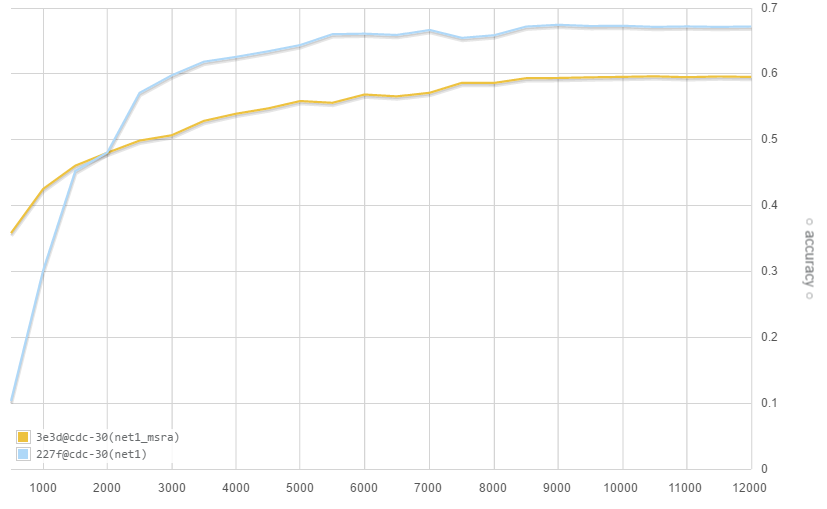
\includegraphics[width=0.9\linewidth]{fig/msra}
    \caption{\small
    Gaussian initialization v.s. msra initialization.
    We can see that msra is worse in this experiment.
    The one with Gaussian has best val accuracy $67.44\%$.
    The one with msra has best val accuracy $59.61\%$.}
    \label{fig:msra}
\end{figure}

\subsection{} % 5.3

Adding BN,
the training is much faster.
The final accuracy also improves.
See Figure~\ref{fig:bn}.

\begin{figure}[ht]
\centering
    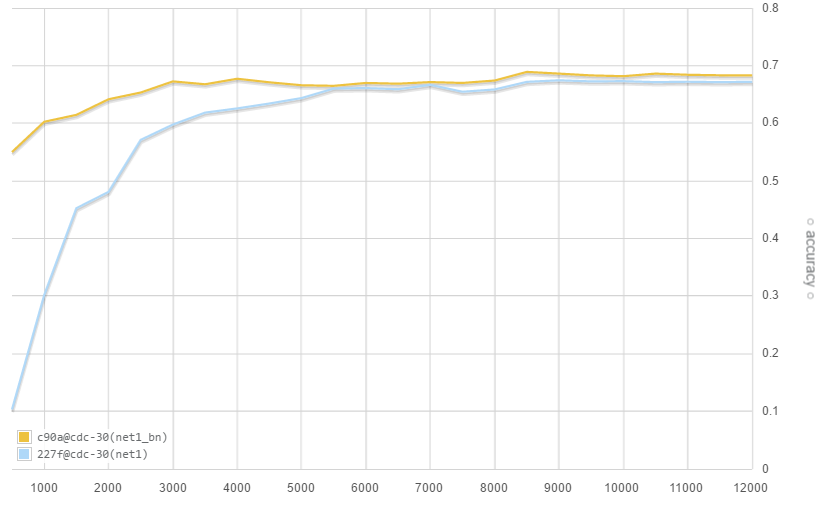
\includegraphics[width=0.9\linewidth]{fig/bn}
    \caption{\small
    Val accuracy with or without BN.
    We can see that BN is very effective in improving
    training speed and test accuracy.
    The one without BN has best val accuracy $67.44\%$.
    The one with BN has best val accuracy $68.91\%$.}
    \label{fig:bn}
\end{figure}

\subsection{} % 5.4

We add augmentation as follows:
Pad 4 pixels around the image and randomly crop to size $32\times 32$.
The result is shown in Figure~\ref{fig:aug}.
*Note*: the implementation of padding and random crop
is using Parrots' code.
Not implemented by self.

\begin{figure}[ht]
\centering
    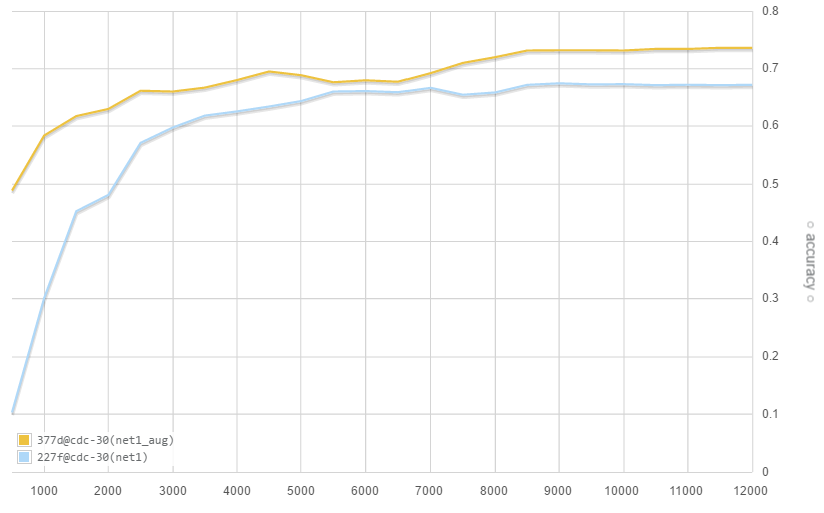
\includegraphics[width=0.9\linewidth]{fig/aug}
    \caption{\small
    Val accuracy with or without augmentation.
    We can see that augmentation is very effective in improving accuracy.
    The one without BN has best val accuracy $67.44\%$.
    The one with BN has best val accuracy $73.61\%$.}
    \label{fig:aug}
\end{figure}
